\section{The accessible entanglement}

Consider an $N$-particle quantum state, with the $N$ particles shared between spatial subregions $A$ and $B$, or Alice and Bob, if you will. If Alice's and Bob's particles are entangled, this entanglement could be used as a resource for real world applications. Nevertheless, by using the traditional Von Neumann or R\'enyi Entanglement entanglement entropy, an overestimated measure of the physically available entanglement is obtained. This happens because for applications that rely on quantum entanglement, the particle number has to be conserved and these traditional measures do not account for this so called Super Selection Rule (SSR). To address the issue, Wiseman and Vaccaro \cite{PhysRevLett.91.097902} proposed a measure that will be referred to here as Accessible Entanglement (originally called Entanglement of Modes by the authors). The accessible entanglement takes into account that the local particle number in $A$ and $B$ has to be conserved, giving a more physically accurate measure of entanglement. A recent generalization of the Renyi Accessible Entanglement Entropy \cite{PhysRevLett.121.150501} allows this entropy to be measured in an experimental setting for arbitrary Renyi Index.\\

In this chapter, analytical results for the accessible entanglement entropy will be presented. 
First, the results will be derived based on the original formulation of the accessible entanglement entropy. After thoroughly going over these derivations, the generalized R\'enyi Accessible Entanglement Entropy will be introduced and analytical results based on this new formulation will also be shown. Finally, numerical results obtained from Exact Diagonalization will be discussed.

	\subsection{Projecting onto subspaces of fixed local particle number}
	
	Knowing the density matrix of subregion $A$ will suffice to calculate spatial Entanglement Entropy. Nevertheless, to get the accessible entanglement, simply knowing $\rho_{A}$ is not enough. The reduced density matrix of $A$, projected onto the subspace of fixed local particle number $n$ is needed. To recap, the spatial R\'enyi Entanglement Entropy is given by:
	
	
\begin{equation}
 S_{\alpha}(\rho_{A}) = \frac{1}{1-\alpha} \log{\Tr{\rho_{A}^{\alpha}}} 
\end{equation}

Where $\alpha$ is the R\'enyi Index and $\rho_{A}$ is the density matrix of subregion $A$. This calculation is still required to get operational entanglement but, as shall be seen, a few extra steps have to be taken to make sure that local particle number conservation is being satisfied. The first of these extra steps will be to project $\rho_{A}$ to subspaces of local particle number. Projection operators can be written as diagonal matrices with ones on the entries corresponding to the subspace for which the projection is desired and zeros for the rest. Knowing this, the projection operators onto subspaces of fixed local particle numbers can be built rather simply. The projected reduced density matrix of  $A$ into the subspace of fixed local particle number $n$ is obtained by:

\begin{equation}
\rho_{A_n} = \frac{1}{P_n} \mathcal{P}_{A_n} \rho_A \mathcal{P}_{A_n}
\label{eq:accessibleEE}
\end{equation}

Where $P_n$ is the probability of measuring an Alice state with $n$ particles and $\mathcal{P}_{A_n}$ is the projection operator onto the subspace of local particle number $n$.

After all this preamble, the accessible entanglement can now be obtained. The operational entanglement is:

\begin{equation}
S_{\alpha}^{\mathrm{acc}}(\rho_A) = \sum_{n} P_n S(\rho_{A_n}) 
\label{eq:accessibleEE}
\end{equation}

Where the sum is carried over all possible local particle numbers that Alice may have. In other words, $n=0,1,...,N-n_{B}$.

In the following section, analytical results of the accessible entanglement entropy at different interaction strength regimes in the $tV$ model are derived.

\section{Analytical results at various regimes of the $tV$ model}
	In the $tV$ model, the state of the system is exactly known in three different interaction strength regimes:
	
	\begin{enumerate} [i)]
		%\item Charged Density Wave (CDW): $V/t \to +\infty $
		%\item Phase Separated Solid:  $V/t \to +\infty $
		%\item First Order Phase Transition: V/t = -2
		
		\item$V/t \to +\infty $
		\item $V/t \to +\infty $
		\item $V/t = -2$
	\end{enumerate}
	
	Starting from the known states at these regimes, analytical values for the operational entanglement were calculated. The results will be discussed in this section.

	\subsection{Infinitely repulsive interaction}
		The state in this limit is known as a charged density wave (CDW). In the occupation number basis, the CDW state is:

\begin{equation}
| \Psi \rangle_{CDW} = \frac{1}{\sqrt{2}} [|101010... \rangle + |010101... \rangle ] 
\end{equation}

Where $1$ denotes that the site is occupied and $0$, that it is vacant. The coefficient before the bracket is a normalization constant. As will be shown, the accessible entanglement for this state is dependent on the parity of the total number of particles $N$. Up next, the result for even N will be derived.

\begin{samepage}
	\subsubsection{Even N}
	In the following calculations, the system will be partitioned into spatial subregions $A$ and $B$, both containing the same number of sites. In other words, if the total number of sites in the $t-V$ chain is $L$, then the partition size will be $l=\frac{L}{2}$. \\
	
In the case of even particle number N, the CDW state will have the same number of particles in each subregion $A$ and $B$:

\begin{equation}
| \Psi \rangle_{N_{Even}} = \frac{1}{\sqrt{2}} [|\underbrace{1010...}_{\frac{N}{2} particles}, \underbrace{1010...}_{\frac{N}{2} particles} \rangle + |\underbrace{0101...}_{\frac{N}{2} particles}, \underbrace{0101...}_{\frac{N}{2} particles} \rangle ] 
\end{equation}

As a reminder, labels left to the comma correspond to spatial subregion $A$, while those to the right correspond to $B$.

The full density matrix $\rho_{AB}$ takes the form:

\begin{equation}
\begin{aligned}
\rho_{AB} &= | \Psi \rangle_{N_{Even}} \langle \Psi |_{N_{Even}} \\
&= \frac{1}{2} |0101...,0101\rangle \langle 0101...,0101... | + \frac{1}{2} |0101...,0101\rangle \langle 1010...,1010... |  \\
&+ \frac{1}{2} |1010...,1010\rangle \langle 0101...,0101... | + \frac{1}{2} |1010...,1010\rangle \langle 1010...,1010... |  \\
\end{aligned}
\label{eq:fullRho_EvenN}
\end{equation}

Recall that to calculate the entanglement entropies, it is necessary to obtain the reduced density matrix of subsystem $A$. Taking the partial trace with respect to $B$, the reduced density matrix of $A$ is obtained:

\begin{equation}
\begin{aligned}
\rho_{A} &= \Tr_{B} \rho_{AB} &= \sum_{n} {}_B \langle n | \Psi \rangle \langle \Psi | n \rangle_{B} \\
\end{aligned}
\end{equation}

The summation above is carried over all possible states that $B$ can be found in. In this case, there are only two possible $B$ states: $n = |0101...\rangle_{B}$ and $n = |1010...\rangle_{B} $. Thus, taking the partial trace respect to $B$ of \ref{eq:fullRho_EvenN}, the reduced density matrix of $A$ becomes:

\begin{equation}
\begin{aligned}
\rho_{A} &= \frac{1}{2} ( | 0101... \rangle_{A} \langle 0101... |_{A} +  | 1010... \rangle_{A} \langle 1010... |_{A} ])\
\end{aligned}
\end{equation}

Notice that some of the terms have vanished due to the orthonormality of the states. At this point, it will be convenient for purposes of illustration to rewrite the reduced density matrix of $A$ in actual matrix form rather than in Dirac or Bra-Ket notation. Following the convention $|0101\dots\rangle_{A}$ and $|1010\dots\rangle_{A}$ for columns and rows from left to right and top to bottom, respectively, the reduced density matrix of $A$ can be written as:

\begin{equation}
\begin{aligned}
\rho_{A} &= \begin{pmatrix}
\frac{1}{2} & 0 \\
0 & \frac{1}{2} \\
\end{pmatrix} \\
\end{aligned}
\end{equation}

For spatial entanglement, $\rho_{A}$ would suffice, but for operational entanglement, the matrix has to now be projected onto the various subspaces or sectors of fixed local particle number in $A$. In this case, both of the states share the same local particle number. That is, the states: $|1010...\rangle_{A}$ and $|0101...\rangle_{A}$ both have local particle number $n = \frac{N}{2}$. Since $\rho_{A}$ only contains entries corresponding to states with the same particle number, no projection is needed. In other words, for this state $\rho_{A} = \rho_{A_{\frac{N}{2}}}$. \\

Taking the partial trace of $\rho_{A} = \rho_{A_{\frac{N}{2}}}$, the probability of measuring a state with local particle number $n = \frac{N}{2} $ is unity, $P_{\frac{N}{2}}=1$.

The projected and normalized reduced density matrix of $A$ is now known and can be substituted into \ref{eq:accessibleEE} to calculate the accessible entanglement entropy:
\begin {align} 
S_{\alpha}^{\mathrm{acc}}(\rho_A) &= \sum_{n} P_n S_{\alpha}(\rho_{A,n}) \nonumber \\
&=  \frac{1}{1-\alpha} P_{\frac{N}{2}} \log{\Tr{\rho_{A,\frac{N}{2}}^{\alpha}}} \nonumber \\
&= \frac{1}{1-\alpha} (1) \log{\Tr{\begin{pmatrix}  (\frac{1}{2})^{\alpha} & 0 \\ 0 & (\frac{1}{2})^{\alpha}   \end{pmatrix}}} \nonumber \\
&= \frac{1}{1-\alpha} \log({\frac{1}{2^{\alpha}} + \frac{1}{2^{\alpha}}}) \nonumber \\
&= \frac{1}{1-\alpha} \log{2^{(1-\alpha)}} \nonumber \\
S_{\alpha}^{\mathrm{acc}}(\rho_A) &= \log{2}
\end {align}

Thus, for even $N$ and $V/t \to + \infty$ , the operational entanglement converges to $\log{2} \approx 0.6931\dots$, independent of the Renyi Index. Up next, the result for odd $N$ will be derived.

	\subsubsection{Odd N}
	
	The most general state is:
	
	\begin{equation}
	| \Psi \rangle_{N_{Odd}} = \frac{1}{\sqrt{2}} [|\underbrace{...101}_{\frac{N+1}{2} particles}, \underbrace{010...}_{\frac{N-1}{2} particles} \rangle + |\underbrace{...010}_{\frac{N-1}{2} particles}, \underbrace{101...}_{\frac{N+1}{2} particles} \rangle ]
	\end{equation}
	
	Note that now when doing an equal spatial bipartition, one of the subregions will have one more particle than the other, unlike the even particle case in which both subregions had the same number of particles. Specifically, one of the subregions will have $\frac{N+1}{2}$ and the other, $\frac{N-1}{2}$. This implies that $\rho_{A}$ will have to be projected onto the space of local particle number $\frac{N+1}{2}$ and then onto $\frac{N-1}{2}$. But before doing that, again the full body density matrix is needed:
	
	\begin{equation}
	\begin{aligned}
\rho_{AB} &= | \Psi \rangle_{N_{Odd}} \langle \Psi |_{N_{Odd}} \\
&= \frac{1}{2} ( |...101,010... \rangle \langle ...101,010... | +  |...101,010... \rangle \langle ...010,101... |  \\
&+  |...010,101... \rangle \langle ...101,010... | + |...010,101... \rangle \langle ...010,101... | )\\
	\end{aligned}
	\end{equation}
	
The possible $B$ states are: $n = | 101... \rangle, | 010... \rangle$ with $\frac{N+1}{2}$ and $\frac{N-1}{2}$ particles, respectively. Taking the partial trace respect to B, the reduced density matrix of $A$ becomes:
	
	\begin{equation}
\begin{aligned}
\rho_{A} &= \frac{1}{2} ( | 101... \rangle_{A} \langle 101... |_{A} +  | 010... \rangle_{A} \langle 010... |_{A} )\\
\end{aligned}
\end{equation}

Once again, it may be more illustrative to rewrite in matrix form. Defining an orthonormal basis $| 101... \rangle_{A}  = \begin{pmatrix} 1 \\ 0\end{pmatrix}$ and $| 010... \rangle_{A}  = \begin{pmatrix} 0 \\ 1\end{pmatrix}$ the reduced density matrix of $A$ becomes:

\begin{equation}
\rho_{A} = 
\begin{pmatrix}
\frac{1}{2} & 0 \\
0 & \frac{1}{2}
\end{pmatrix}
\end{equation}

The simple projection operators onto $\frac{N+1}{2}$ and $\frac{N-1}{2}$ particle space in this basis are:

\begin{equation}
\mathcal{P}_{A_{\frac{N+1}{2}}} = \begin{pmatrix} 1 & 0 \\ 0 & 0 \end{pmatrix} , 
\mathcal{P}_{\frac{N-1}{2}} = \begin{pmatrix} 0 & 0 \\ 0 & 1 \end{pmatrix} 
\end{equation}

Applying these projections to $\rho_{A}$ and choosing the probability such that the trace of each matrix is unity (normalization), the projected reduced density matrices become:

\begin{equation}
\rho_{A,{\frac{N+1}{2}}} = \begin{pmatrix} 1 & 0 \\ 0 & 0 \end{pmatrix}  \text{ with probability } P_{\frac{N+1}{2}} = \frac{1}{2}
\end{equation}

and 

\begin{equation}
\rho_{A,{\frac{N-1}{2}}} = \begin{pmatrix} 0 & 0 \\ 0 & 1 \end{pmatrix}  \text{ with probability } P_{\frac{N-1}{2}} = \frac{1}{2}
\end{equation}

Substituting into the accessible entanglement equation (\ref{eq:accessibleEE}):

\begin {align} 
S_{\alpha}^{acc}(\rho_A) &= \sum_{n} P_n S_{\alpha}(\rho_{A,n}) \nonumber \\
&= (\frac{1}{2})\frac{1}{1-\alpha} \log{\Tr{\rho_{A,\frac{N+1}{2}}^{\alpha}}} + (\frac{1}{2})\frac{1}{1-\alpha} \log{\Tr{\rho_{A,\frac{N-1}{2}}^{\alpha}}} \nonumber \\
&=\frac{1}{2-2\alpha}[ \log{\Tr{\begin{pmatrix}  1^{\alpha} & 0 \\ 0 & 0   \end{pmatrix}}} + \log{\Tr{\begin{pmatrix}  0 & 0 \\ 0 & 1^{\alpha}   \end{pmatrix}}}] \nonumber \\
&=  \frac{1}{2-2\alpha}[ \underbrace{\log{1} + \log{1}}_{=0} ] \nonumber \\
S_{\alpha}^{acc}(\rho_A) &= 0
\end {align}

Therefore, the operational entanglement vanishes in the infinite repulsion limit ($V/t \to + \infty$) with odd number of total particles in the system.

The results for the accessible entanglement in the infinitely repulsive limit can then be summarized as:

\begin{equation}
\lim_{V \to + \infty} S_{\alpha}^{acc} =
\begin{cases}
\log{2}  & \text{if }N\text{ is even} \\
0 & \text{if }N\text{ is odd}
\end{cases}
\end{equation}

\end{samepage}

	\subsection{Infinitely attractive interaction}
	In this section, an analytical result will be derived at half-filling ($L = 2N$) and partition size equal to half the number of sites ($\ell = \frac{L}{2}$) for $V/t \to - \infty$. After arriving to the half-filling result, a general result, for any filling fraction and partition size, will be also derived. 
	
	\subsubsection{Half-filling}
	In the infinitely attractive regime of the $tV$ model, $V/t \to -\infty$, the fermions cluster together. The most general state in this regime is:
	
\begin{equation}
\begin{aligned}	
| \Psi \rangle_{PSS} = \frac{1}{\sqrt{L}} [ | \underbrace{111...111}_{N particles} , \underbrace{000...000}_{N vacancies} \rangle + |011...111, 100...000 \rangle + |001...111, 110...000 \rangle  \\
+ ...  + |\underbrace{000...000}_{N vacancies}, \underbrace{111...111}_{N particles} \rangle + |100...000, 011...111 \rangle + ... |111...110, 000...001 \rangle ]
\end{aligned}
\end{equation}

This state is known as a phase separated solid (PSS). There are a total of $L$ possible configurations, hence the normalization constant $\frac{1}{\sqrt{L}}$. 

In an effort to simplify the notation while keeping the calculation general, the $A$ or $B$ states will be relabeled as:

\begin {align*}
&| 111...111 \rangle_{A} \to | N \rangle \\
&| 011...111 \rangle_{A} \to | N-1 \rangle \\
&| 001...111 \rangle_{A} \to | N-2 \rangle \\
&\vdots \\
&| 000...011 \rangle_{A} \to | 2 \rangle \\
&| 000...001 \rangle_{A} \to | 1 \rangle \\
&| 000...000 \rangle_{A} \to | 0 \rangle 
\end {align*}

There is still one flaw with this notation. A $| N-1 \rangle $ state could represent either $| 011...111 \rangle $ or $|111...110 \rangle $. In other words, even though they have the same local particle number $N-1$, the configurations themselves are different. One way in which this problem can be circumvented is by adding a subscript to the label to represent distinct configurations. Since particle number will only be shared between two distinct particle configurations, using subscripts of $1$ and $2$ seems natural. For example: $| 011...111 \rangle \to | (N-1)_1 \rangle$ and $|111...110 \rangle \to | (N-1)_2 \rangle$. $|\Psi\rangle_{PSS}$ now becomes:

\begin{equation}
\label{eq:PSS_State}
| \Psi \rangle_{PSS} = \frac{1}{\sqrt{L}} [ |N, 0 \rangle + |(N-1)_1, 1_1 \rangle + |(N-2)_1, 2_1 \rangle  
+ ...  + |0, N \rangle + |1_2, (N-1)_2 \rangle + ... |(N-1)_2, 1_2 \rangle ]
\end{equation}

Taking the outer product of Eq. \ref{eq:PSS_State} with itself, the full body density matrix is obtained:

\begin{equation}
\label{eq:PSS_Matrix}
\rho_{AB} = | \Psi \rangle_{PSS} \langle \Psi |_{PSS} = 
\begin{pmatrix} 
\frac{1}{L} & \frac{1}{L} & ... & \frac{1}{L} \\
\frac{1}{L} & \frac{1}{L} & ... & \frac{1}{L} \\
\vdots & \vdots & \vdots & \vdots \\
\frac{1}{L} & \frac{1}{L} & ... & \frac{1}{L} \\
\end{pmatrix}
\end{equation}

The full body density matrix is of size $LxL$ with all entries equal to $\frac{1}{L}$. Before proceeding, the basis of this matrix should be described. Columns (from left to right) and rows (from top to bottom) are arranged as: $| N, 0 \rangle , |0, N \rangle , | (N-1)_1, 1_1 \rangle, |(N-1)_2, 1_2 \rangle , | (N-2)_1, 2_1 \rangle , | (N-2)_2, 2_2 \rangle , ... , |2_1, (N-2)_1 \rangle , \rangle, |2_2, (N-2)_2 \rangle , \rangle, |1_1, (N-1)_1 \rangle , \rangle, |1_2, (N-1)_2 \rangle  $. Notice that configurations that share local particle number have been paired up next to each other in the prescribed ordering scheme. The first two states are exceptions, as their subregions never share the same local particle number with subregions of any other state. Now that the basis has been explained, it's time to get the reduced density matrix of $A$. \\
\\
Taking the partial trace with respect to $B$ of Eq. \ref{eq:PSS_Matrix}, the reduced density matrix becomes:

\begin{equation}
\rho_{A} = \begin{pmatrix}
\frac{1}{L} & 0 &... & 0 & 0 \\
0 & \frac{1}{L} & ... & 0 & 0 \\
\vdots & \vdots & \ddots & \vdots & \vdots \\
0 & 0 & ... & \frac{1}{L} & 0 \\
0 & 0 & ... & 0 & \frac{1}{L} \\
\end{pmatrix}
\end{equation}

In the above matrix, the rows and columns correspond to the following configurations and in the following order: $| N \rangle_{A} , |0 \rangle_{A} , | (N-1)_1 \rangle_{A}, |(N-1)_2 \rangle_{A} , | (N-2)_1 \rangle_{A} , | (N-2)_2 \rangle_{A} , ... , |2_1 \rangle_{A} , |2_2 \rangle_{A} , |1_1 \rangle_{A} , |1_2 \rangle_{A} $.

Now, $\rho_{A}$ has to be projected onto the subspaces of local particle numbers. The allowed local particle numbers are: $n = N, N-1, N-2 .... 2, 1, 0$. So a total of $N+1$ projections need to be done.

The projection operators for $n=0$ and $n=N$ become:

\begin{equation}
\mathcal{P}_{N} = \begin{pmatrix} 
1 & 0 &... & 0 & 0 \\
0 & 0 & ... & 0 & 0 \\
\vdots & \vdots & \ddots & \vdots & \vdots \\
0 & 0 & ... & 0 & 0 \\
0 & 0 & ... & 0 & 0 \\
\end{pmatrix} , 
\mathcal{P}_{0} = \begin{pmatrix} 
0 & 0 &... & 0 & 0 \\
0 & 1 & ... & 0 & 0 \\
\vdots & \vdots & \ddots & \vdots & \vdots \\
0 & 0 & ... & 0 & 0 \\
0 & 0 & ... & 0 & 0 \\
\end{pmatrix}
\end{equation}

For the remaining $N - 1$ states, there will be two consecutive non-zero entries in the diagonal corresponding to the different fixed local particle number pairs. For example:

\begin{equation}
\mathcal{P}_{N-1} = \begin{pmatrix} 
0 \\
& 0 \\
& & 1 \\
& & & 1 \\
& & & &  0 \\
& & & & & 0 \\
& & & & &  & \ddots \\
& & & & & & &  0 \\
& & & & & & & &  0 \\
\end{pmatrix}
\nonumber
\end{equation}

\begin{equation}
\mathcal{P}_{N-2} = \begin{pmatrix} 
0 \\
& 0 \\
& & 0 \\
& & & 0 \\
& & & &  1 \\
& & & & & 1 \\
& & & & &  & \ddots \\
& & & & & & &  0 \\
& & & & & & & &  0 \\
\end{pmatrix}
,
\mathcal{P}_{1} = \begin{pmatrix} 
0 \\
& 0 \\
& & 0 \\
& & & 0 \\
& & & &  0 \\
& & & & & 0 \\
& & & & & & \ddots \\
& & & & & & &  1 \\
& & & & & & & &  1 \\
\end{pmatrix}
\end{equation} \\
\\

Notice from the form of the projection operators that the projected reduced density matrices will be similar to each other but with the two non-zero entries shifted correspondingly in the diagonal. Thus, taking the projection onto $n=N-1$ of $\rho_{A}$, the projected reduced density matrix of this particle sector becomes:

\begin{equation}
\begin{aligned}
\rho_{A,N-1} &= \frac{1}{P_{N-1}} \hat{\Pi}_{N-1} \rho_{A} \hat{\Pi}_{N-1} \\
\rho_{A,N-1} &= \frac{1}{P_{N-1}} \begin{pmatrix} 
0 \\
& 0 \\
& & \frac{1}{L} \\
& & & \frac{1}{L} \\
& & & &  0 \\
& & & & & 0 \\
& & & & &  & \ddots \\
& & & & & & &  0 \\
& & & & & & & &  0 \\
\end{pmatrix} 
\end{aligned}
\end{equation}

The probability of measuring a state with local particle number $N-1$ can be obtained from normalization:

\begin{equation}
\Tr{\rho_{A,N-1}} = 1 \implies \frac{1}{P_{N-1}}\frac{2}{L} = 1 \implies P_{N-1} = \frac{2}{L}
\end{equation}

Thus, the normalized projection onto $n=N-1$ of $\rho_{A}$ is:

\begin{equation}
\rho_{A,N-1} = \begin{pmatrix} 
0 \\
& 0 \\
& & \frac{1}{2} \\
& & & \frac{1}{2} \\
& & & &  0 \\
& & & & & 0 \\
& & & & &  & \ddots \\
& & & & & & &  0 \\
& & & & & & & &  0 \\
\end{pmatrix} ; \text{ with probability } P_{N-1} = \frac{2}{L}
\end{equation}

For $n = N-2$:
\begin{equation}
 \rho_{A,N-2} = \begin{pmatrix} 
0 \\
& 0 \\
& & 0  \\
& & & 0 \\
& & & &  \frac{1}{2} \\
& & & & & \frac{1}{2} \\
& & & & &  & \ddots \\
& & & & & & &  0 \\
& & & & & & & &  0 \\
\end{pmatrix} ; \text{ with probability } P_{N-2} = \frac{2}{L}
\end{equation}

and so on and so forth. \\
\\
Similarly, $\rho_{A,N}$ and $\rho_{A,0}$ become:
\begin{equation}
\rho_{A,N} = \begin{pmatrix} 
1 \\
& 0 \\
& & 0  \\
& & & 0 \\
& & & &  0 \\
& & & & & 0 \\
& & & & &  & \ddots \\
& & & & & & &  0 \\
& & & & & & & &  0 \\
\end{pmatrix} ,
\rho_{A,0} = \begin{pmatrix} 
0 \\
& 1 \\
& & 0  \\
& & & 0 \\
& & & &  0 \\
& & & & & 0 \\
& & & & &  & \ddots \\
& & & & & & &  0 \\
& & & & & & & &  0 \\
\end{pmatrix} 
\end{equation}

with probabilities $P_{N} = P_{0} = \frac{1}{L}$ \\

Finally, the accessible entanglement is:

\begin{align} 
S_{\alpha}^{acc}(\rho_A) &= \sum_{n} P_n S_{\alpha}(\rho_{A,n}) \nonumber \\
&= \frac{1}{1-\alpha}[\frac{1}{L} \log{\Tr{\rho_{A,N}^\alpha}} + \frac{1}{L} \log{\Tr{\rho_{A,0}^\alpha}} + \frac{2}{L} \log{\Tr{\rho_{A,N-1}^\alpha}} \nonumber \\
&+ \frac{2}{L} \log{\Tr{\rho_{A,N-2}^\alpha}} + \dots +\frac{2}{L} \log{\Tr{\rho_{A,2}^\alpha}} + \frac{2}{L} \log{\Tr{\rho_{A,1}^\alpha}} ] \nonumber \\
&= \frac{1}{L-L\alpha}[ \underbrace{\log{1}}_{=0} +  \underbrace{\log{1}}_{=0} + 2 \log({\frac{1}{2^\alpha}+\frac{1}{2^\alpha}}) \nonumber \\
&+ 2 \log({\frac{1}{2^\alpha}+\frac{1}{2^\alpha}})+ \dots + 2 \log({\frac{1}{2^\alpha}+\frac{1}{2^\alpha}}) + 2 \log({\frac{1}{2^\alpha}+\frac{1}{2^\alpha}}) ] \nonumber \\
&= \frac{2}{L-L\alpha}\underbrace{[\log{2^{(1-\alpha)}} + \log{2^{(1-\alpha)}} + \dots + \log{2^{(1-\alpha)}} + \log{2^{(1-\alpha)}}}_{N - 1 \text{ or } \frac{L}{2}-1\text{ total terms }}] \nonumber \\
&= (\frac{L}{2}-1)(\frac{2}{L})\log{2^\frac{1-\alpha}{1-\alpha}} \nonumber \\
&= (\frac{L-2}{2})(\frac{2}{L})\log{2} ; \text{ recall that } L = 2N \nonumber \\
S_{\alpha}^{acc}(\rho_A) &= \frac{N-1}{N}\log{2}
\end{align}

\subsubsection{Analytical result for any filling fraction and partition size}

The analytical result obtained above for the accessible entanglement entropy in the infinitely attractive regime corresponds to the special case of half-filling ($N = \frac{L}{2}$) and equal spatial bipartitions ($\ell_{A} = \ell_{B} = \frac{L}{2}$). Nevertheless, a generalized result can be obtained for any filling fraction and partition size by counting the number of projected reduced density matrices ($\rho_{A,n}$) that will contribute to the accessible entanglement. As it will be shown, the number of contributing matrices will depend on how the quantities $\ell_{A}, \ell_{B}, N \text{ } \&  \text{ }N^{c} = L-N$ relate to each other. Demonstration of the following cases will suffice to get the general result:

\begin{align}
&i) \ell_{A} < N < \ell_{B} \nonumber \\
&ii) \ell_{B} < N < \ell_{A} \nonumber \\
&iii)  N < \ell_{A} < \ell_{B} \nonumber \\
&iv) \ell_{A} < \ell_{B} < N \nonumber
\end{align}

These four cases actually imply other cases and, in the end, all possible relations between the four parameters should be covered. \\

Case $i)$ $\ell_{A} < N < \ell_{B}$:

The condition here is that the size of the subregion $A$ should be less than the total number of particles $N$ and the size of the subregion $B$ should be greater than both of these quantities. Under such conditions, particle configurations in which $B$ is empty are not possible, since $A$ is too small too fit them all. Two other configurations that will not contribute to the operational entanglement are when $A$ is full ($n_{A} = \ell_{A}$) and when it is empty ($n_{A} = 0$). There is only one possible way of distributing the particles in partition $A$ if it is full and likewise if it is empty. As it was seen in the previous section, then the corresponding projected reduced density matrices $\rho_{A,\ell_{A}}$ and $\rho_{A,0}$ have only one nonzero eigenvalue which, after normalization, becomes 1. Thus, $\ln \rho_{A,\ell_{A}}^{\alpha} = \ln \rho_{A,0}^{\alpha} = 0$. There are a total of $\ell_{A}+1$ possible local particle numbers ($n_{A}$) and since $n_{A} = \ell_{A}$ and $n_{A} = 0$ do not contribute, there are actually $\ell_{A}-1$ contributing projected reduced density matrices. All such projected density matrix will have the form:

\begin{equation}
\rho_{A,n} = \begin{pmatrix} 

\frac{1}{L} & 0 \\
0 & \frac{1}{L} \\

\end{pmatrix}
\end{equation}

The two diagonal elements come from the two configurations that have the same local particle number $n$. Technically, these projected reduced density matrices are larger, since the basis includes configurations with all possible local particle numbers. Nevertheless, rows and columns that only have zero entries have been thrown out for compactness. Normalizing, the reduced density matrices become:

\begin{equation}
\rho_{A,n} = \frac{1}{P_n} \begin{pmatrix} 

\frac{1}{2} & 0 \\
0 & \frac{1}{2} \\

\end{pmatrix} ; P_n = \frac{2}{L}
\end{equation}

Thus, the accessible entanglement becomes:

\begin{equation}
S_{\alpha}^{acc} (\ell_A, L) = (\ell_{A} - 1) \frac{2}{L} \ln{2}
\end{equation}

Case $ii)$ $\ell_{B} < N < \ell_{A}$:

This time, partition $B$ is the one that can never be empty. Barring that, the argument is exactly the same as $i)$ and thus:

\begin{equation}
S_{\alpha}^{op} (\ell_{B}, L) = (\ell_{B} - 1) \frac{2}{L} \ln{2}
\end{equation}

Case $iii)$ $N < \ell_{A} < \ell_{B}$:

In contrast to $i)$ and $ii)$, now the particles may all be in $A$ or all in $B$. Nevertheless, in such instances, there is only a single possible configuration of the other partition, that in which it's empty. Thus, the projected reduced density matrices $\rho_{A,N}$ and $\rho_{A,0}$ have only one nonzero eigenvalue and, thus, do not contribute to the operational entanglement since this eigenvalue will reduce to unity after normalization. Barring these two, there are then $N-1$ projected reduced density matrices that do contribute. They all have the same form as the ones of $i)$ and $ii)$, that is, $2x2$ diagonal matrices (after throwing out all unnecessary zeroes) with 2 eigenvalues equal to $\frac{1}{2}$ (after normalizing) and probabilities $P_n = \frac{2}{L}$. Thus:

\begin{equation}
S_{\alpha}^{op} (N, L) = (N - 1) \frac{2}{L} \ln{2}
\end{equation}

Case $iv)$ $\ell_{A} < \ell_{B} < N$:

Here, no partition will ever be empty. The maximum allowed particle number in $A$ is going to be $n_{A} = \ell_{A}$ and the smallest one, $n_{A} = N - \ell_{B}$. The partition size of $B$ is subtracted from $N$ because the minimum $n_A$ corresponds to a fully occupied partition $B$, that is $n_B = \ell_B$. The 'leftover' particles on $A$ will hence be the total particle number minus those fully occupying $B$. Notice in all the previous examples that the total number of projected reduced density matrix is equal to the difference between max and min allowed particle number $n_A$ plus 1. That is:

\begin{equation}
\text{Total Projected Reduced Density Matrices} = (n_A)_{max} - (n_A)_{min} + 1
\end{equation}

And for this case,

 \begin{align}
\text{Total Projected Reduced Density Matrices} &= (n_A)_{max} - (n_A)_{min} + 1 \nonumber \\
&= \ell_A - (N-\ell_B) + 1 \nonumber \\
&= \underbrace{\ell_A + \ell_B}_{L} - N + 1 \nonumber \\
\text{Total Projected Reduced Density Matrices} &= L - N + 1
\end{align}

Let $L-N \equiv N^c$. The total number of contributing projected reduced density matrices is:

\begin{align}
\text{Contributing Matrices} &= \text{Total Matrices} - 2 \nonumber \\
&= (N^c + 1) - 2 \nonumber \\
\text{Contributing Matrices} &= N^c - 1 \\
\end{align}

the accessible entanglement then becomes:

\begin{equation}
S_\alpha^{op}(N^c,L) = (N^c - 1) \frac{2}{L} \ln{2}
\end{equation}

The accessible entanglement at the infinitely attractive regime has now been obtained for conditions $i)-iv)$. Notice that it always has the form:

\begin{equation}
S_\alpha^{op}(x,L) = (x - 1) \frac{2}{L} \ln{2}
\end{equation}

where $x$ could be  $\ell_A, \ell_B, N$ or $N^c$. But how to determine which of these variables to choose? Recalling that $L-N = N^c, L-\ell_A = \ell_B$ and $L-\ell_B = \ell_A$, extra inequalities can be obtained from $i)-iv)$ that relate the four variables:

\begin{align}
& i) \ell_{A} < N < \ell_{B} \implies \ell_{B} > N^c > \ell_{A} \implies \ell_{A} \text{ is the smallest} \nonumber \\
& ii) \ell_{B} < N < \ell_{A} \implies \ell_{A} > N^c > \ell_{B} \implies \ell_{B} \text{ is the smallest} \nonumber \\
& iii)  N < \ell_{A} < \ell_{B} \implies N^c > \ell_{B} > \ell_{A} \implies N \text{ is the smallest} \nonumber \\
& iv) \ell_{A} < \ell_{B} < N \implies \ell_{B} > \ell_{A} > N^c \implies N^c \text{ is the smallest} \nonumber 
\end{align}

From the above set of inequalities, note that the smallest between the four variables in each case, also happens to be the variable that is substituted for $x$. Thus, in a more compact form, the generalized operational entanglement at the infinitely attractive regime is:

\begin{equation}
S_\alpha^{op}(x,L) = \frac{2(x-1)}{L} \ln{2} ; \text{ where } x = \min{\ell_A, \ell_B, N, N^c}
\end{equation}

	\subsection{First order phase transition}
	
At $\frac{V}{t} = -2$, the $tV$-Model undergoes a first order phase transition from Luttinger Liquid to Phase Separated Solid. The operational entanglement at this interaction strength vanishes and then suddenly increases and converges to the previously derived limit ($\frac{N-1}{N}\ln{2}$) as the attraction gets stronger. In this section, it will be shown that the operational entanglement vanishes at the first order phase transition.

At $\frac{V}{t}=-2$ and half-filling ($N=\frac{L}{2}$), the state of the system is an equiprobable superposition of all possible configurations. There are a total of ${L}\choose{N}$ possible configurations. Thus, the general state can be written as: 

\begin{equation} 
|\Psi \rangle = \frac{1}{\sqrt{{L}\choose{N}}} \sum_{i=1}^{{L}\choose{N}} | \phi_{i} \rangle
\end{equation}

where $|\phi_{i}\rangle$ is the set of all configurations of $N$ fermions on $L$ sites and the pre-factor is a normalization constant. Now that the state at $\frac{V}{t}=-2$ is known, the full and, hence, reduced density matrices can be obtained. Up next, their resulting general structure will be discussed.

For simplicity, let $\frac{1}{\sqrt{{L}\choose{N}}} \equiv C$. For particle sub-sectors of $n_A = 0$ and $n_A = N$, the projected reduced density matrices become:

\begin{equation}
\rho_{A,N} = \frac{1}{P_{N}} \begin{pmatrix}
C & \dots & 0 \\ 
\vdots & 0 & \vdots \\
0 & \dots & 0 \\
\end{pmatrix}
\end{equation}

with probability $P_{N} = C$. And, 

\begin{equation}
\rho_{A,0} = \frac{1}{P_{0}} \begin{pmatrix}
0 & \dots & 0 \\ 
\vdots & 0 & \vdots \\
0 & \dots & C \\
\end{pmatrix}
\end{equation}

also with probability $P_{0} = C$.

For particle number sub-sectors of $1 \leq n \leq N-1$, the projected reduced density matrices become square matrices of size $NxN$ with all entries being $NC^2$:

\begin{equation}
\rho_{A,n} = \frac{1}{P_{n}} \begin{pmatrix}
NC^2 & \dots & NC^2 \\ 
\vdots & NC^2 & \vdots \\
NC^2 & \dots & NC^2
\end{pmatrix}
\end{equation}

with probabilities $P_{n}=N(NC^2)=N^2C^2$.

In summary, the normalized projected reduced density matrices are:

\begin{equation}
\rho_{A,N} = \frac{1}{P_{N}} \begin{pmatrix}
1 & \dots & 0 \\ 
\vdots & 0 & \vdots \\
0 & \dots & 0 \\
\end{pmatrix}, P_{N}=C 
\end{equation}
\begin{equation}
 \rho_{A,0} = \frac{1}{P_{N}} \begin{pmatrix}
0 & \dots & 0 \\ 
\vdots & 0 & \vdots \\
0 & \dots & 1 \\
\end{pmatrix}, P_{0}=C 
\end{equation}
\begin{equation}
\rho_{A,n} = \frac{1}{P_{n}} \begin{pmatrix}
\frac{1}{N} & \dots & \frac{1}{N} \\ 
\vdots & \frac{1}{N} & \vdots \\
\frac{1}{N} & \dots & \frac{1}{N}
\end{pmatrix}, P_{n}=N^2C^2 
\end{equation}

Recall the definition of the accessible (R\'enyi) entanglement entropy:

\[S_{\alpha}^{acc}(\rho_{A}) = \sum_{n} P_{n}S(\rho_{A,n})\]

where $S_{\alpha}(\rho_A) = \frac{1}{1-\alpha} \log{\Tr{(\rho_A^{\alpha})}}$
\\
Expanding the sum:

\begin{align}
S_{\alpha}^{acc}(\rho_{A}) &= P_{0} \log{\Tr{(\rho_{A,0}^{\alpha})}} + P_{N} \log{\Tr{(\rho_{A,N}^{\alpha})}} + \sum_{n=1}^{N-1} P_{n} \log{\Tr{(\rho_{A,n}^{\alpha})}} \nonumber \\
&= C \log{1} + C \log{1} + N^2C^2 \sum_{n=1}^{N-1} \log{N(\frac{1}{N})}  \nonumber \\
&= N^2C^2 \sum_{n=1}^{N-1} \log{1} \nonumber \\
S_{\alpha}^{acc}(\rho_{A}) &= 0 
\end{align}

Thus, the accessible entanglement vanishes at the first order phase transition. \\

Analytical results have been obtained in three regimes of the $tV$ Model, namely: $V/t \to + \infty$, $V/t \to - \infty$ and $V/t = -2$. In the next section a generalization of the R\'enyi Accessible Entanglement Entropy will be discussed and the analytical results at the aforementioned limits will be shown.

\section{Generalized R\'enyi Accessible Entanglement Entropy}

Computing the accessible entanglement for a many-body system is a difficult task for $\alpha=1$, as full state tomography is required to reconstruct the density matrix $\rho$. However, for integer values with $\alpha > 1$ a replica trick can be used to recast $\mathrm{Tr} \rho_A^\alpha$ as the expectation value of some local operator \cite{Calabrese:2004hl}. This advance has led to a boon of new entanglement results using both computational \cite{Hastings:2010dc, Humeniuk:2012cq, McMinis:2013dp, Herdman:2014ey, Drut:2015fs} and experimental \cite{Daley:2012bd, Islam:2015cm, Kaufman:2016ep, Pichler:2016ec, Linke:2017tf, Lukin:2018wg} methods.  Motivated by this progress, two of us recently generalized the accessible entanglement to the case of \ren entropies with $\alpha \ne 1$ and found that \cite{Barghathi:2018oe}:
%
\begin{equation}
S_{\alpha}^{{\rm acc}} (\rho_A) = \frac{\alpha}{1-\alpha}\ln\left[ \sum_{n} P_n \mathrm{e}^{\frac{1-\alpha}{\alpha} S_{\alpha}(\rho_{A_n})}\right]
\label{eq:S_alpha_acc}
\end{equation} 
%
% which reproduces Eq.~\eqref{eq:S1acc} in the limit $\alpha \to 1$. While not physically transparent in this form, the modification from the $\alpha=1$ case results from replacing the geometric mean in Eq.~\eqref{eq:S1acc} with a general power mean whose form is constrained by the physical requirement that $0 \le \Delta S_\alpha \le \ln (N+1)$.  It can also be interpreted as the quantum generalization of the conditional classical \ren entropy \cite{Cachin97entropymeasures,GolshaniPashaYari:2009,Hayashi:2011,SKORIC:2011el,FehrBerens2014} subject to physical constraints \cite{Barghathi:2018oe}. The arguments leading to Eq.~\eqref{eq:DS1H1} can also be generalized leading to 
which reproduces Eq.~\eqref{eq:S1acc} in the limit $\alpha \to 1$. While not physically transparent in this form, the modification from the $\alpha=1$ case results from replacing the geometric mean in Eq.~\eqref{eq:S1acc} with a general power mean whose form is constrained by the physical requirement that
%
\begin{equation}
 0 \le \Delta S_\alpha \le \ln (N+1)
\label{eq:DeltaS_alpha_inq}
\end{equation}
%
where the upper bound is equal to the support of $P_n$. \Eqref{eq:S_alpha_acc} can also be interpreted as the quantum generalization of the conditional classical \ren entropy \cite{Cachin97entropymeasures,GolshaniPashaYari:2009,Hayashi:2011,SKORIC:2011el,FehrBerens2014}, subject to physical constraints \cite{Barghathi:2018oe}. The arguments leading to Eq.~\eqref{eq:DS1H1} can then be generalized (see the supplemental material of Ref.~[\onlinecite{Barghathi:2018oe}]) leading to 
%
\begin{equation}
    \Delta S_{\alpha}\equiv  S_{\alpha} - S_{\alpha}^{{\rm acc}} = H_{{1}/{\alpha}}\left(\{P_{n,\alpha}\}\right)
\label{eq:S_alpha_acc5}
\end{equation}
%
where we introduce the classical \ren entropy of $P_n$
%
\begin{equation}
    H_{\alpha}\left(\{P_n\}\right)=\frac{1}{1-\alpha}\ln\sum_n P_n^{\alpha} 
\label{eq:Halpha}
\end{equation}
%
and
%
\begin{equation}
    P_{n,\alpha}=\frac{\Tr\, \left[{\mathcal{P}}_{A_{n}} \rho_A^{\alpha} {\mathcal{P}}_{A_{n}}\right]}{\Tr\, \rho_A^{\alpha}}=\frac{ P_n^\alpha\Tr\, \rho_{A_n}^{\alpha}}{\Tr\, \rho_A^{\alpha}}
\label{eq:Pna}
\end{equation}
%
can be interpreted as a normalization of partial traces of $\rho_A^{\alpha}$, where the SSR fixing the total particle number leads to $\Tr\, \rho_A^{\alpha}=\sum_n \Tr\, \left[{\mathcal{P}}_{A_{n}} \rho_A^{\alpha} {\mathcal{P}}_{A_{n}}\right]$ and thus guarantees the normalization of $P_{n,\alpha}$. Note that we have defined $P_{n,1} \equiv P_n$ for notational consistency. For brevity, let $H_{\alpha}(\{P_n\}) \equiv H_{\alpha}$ from here onwards. 

Writing the difference $\Delta S_{\alpha}$ as the classical \ren entropy of the fictitious probability distribution $P_{n,\alpha}$, simplifies the calculation of $\Delta S_{\alpha}$ and clarifies its properties, e.g., the fact that $H_{\alpha}$  is positive and bounded from above by $ H_{0}=\ln(N+1)$ guarantees that $\Delta S_{\alpha}$ satisfies the physical requirement in \Eqref{eq:DeltaS_alpha_inq}. \cite{Barghathi:2018oe} In addition, $P_{n,\alpha}$ is fully determined by $P_n$ and the full and the projected traces of $\rho_A^{\alpha}$, i.e.~$\Tr\, \rho_{A}^{\alpha}$ and $\Tr\, \rho_{A_n}^{\alpha}$, which can be measured using the experimental and numerical methods mentioned above.

\section{Numerical Results}
	\subsection{Operational entanglement as a function of interaction strength}
		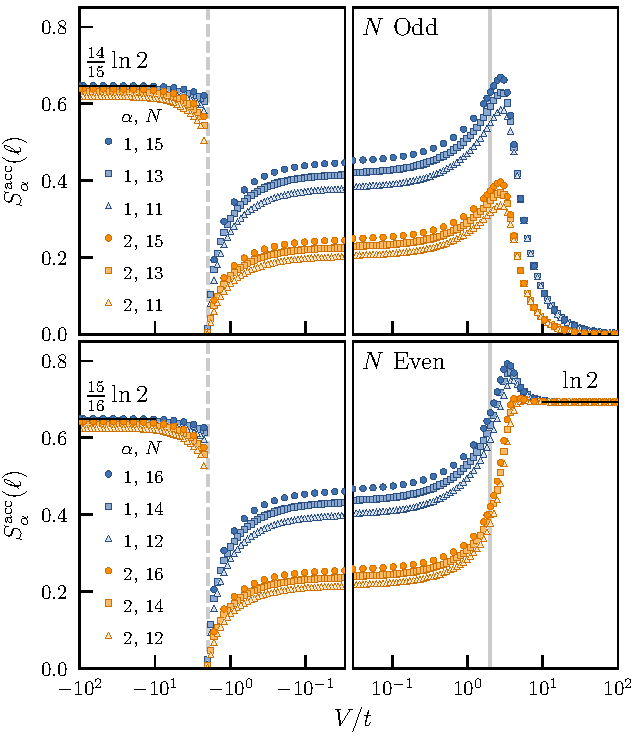
\includegraphics{operationalEntanglementEntropies_SOP5}
		
	\subsection{}
		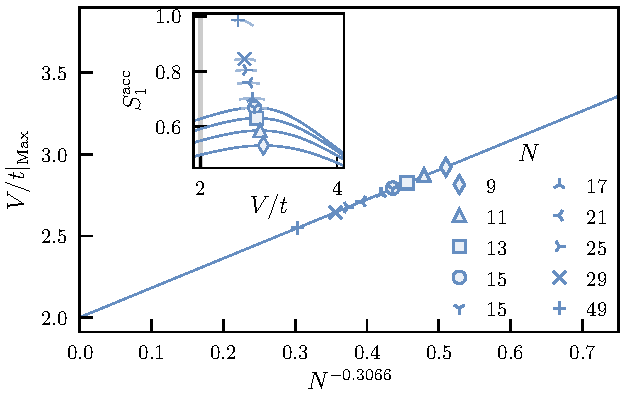
\includegraphics{peakScalingOddN.pdf}
		
	\subsection{}
		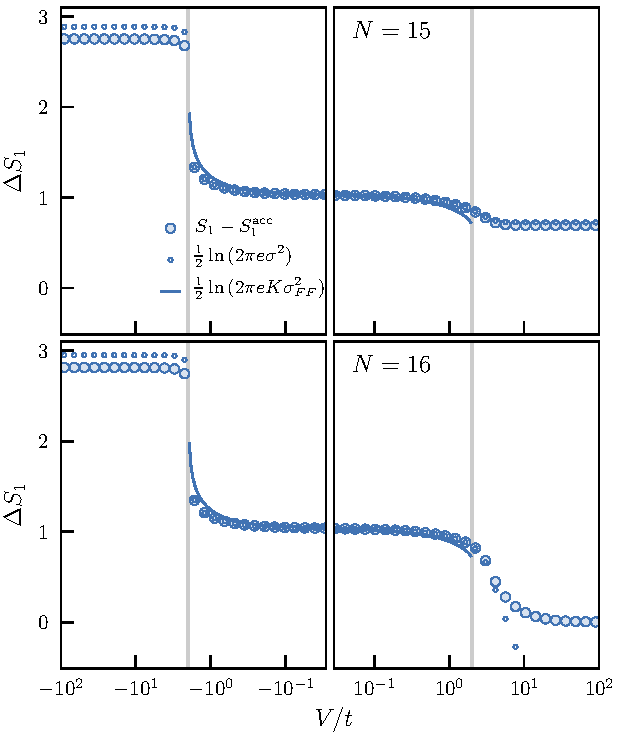
\includegraphics{deltaS1_N15N16}
		
	\subsection{}
		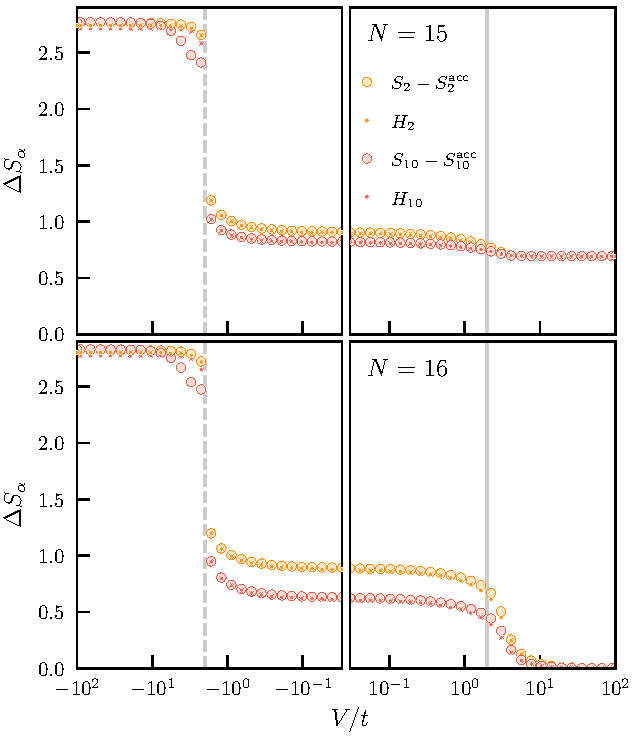
\includegraphics{higherAlphaDeltaS_N15N16.pdf}

	\subsection{}
		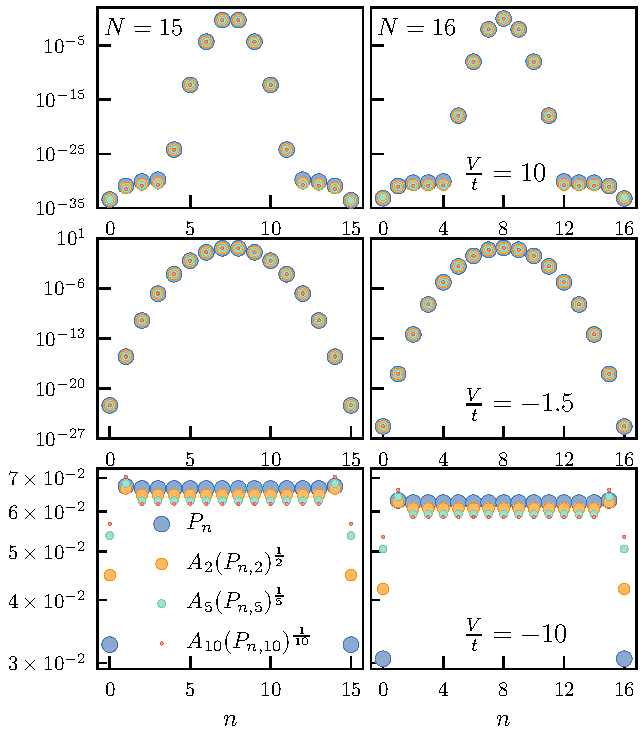
\includegraphics{alphaCollapse}

	\subsection{}
		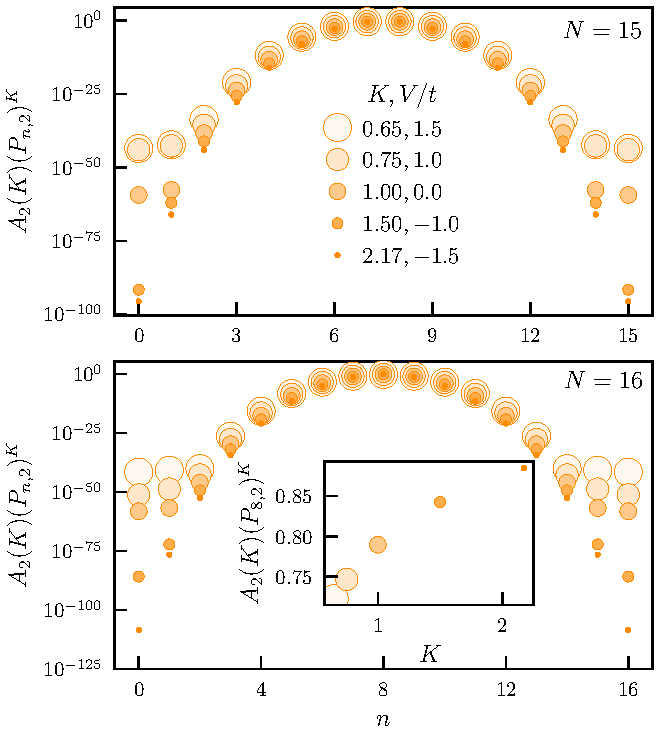
\includegraphics{TLLCollapse}
				
	\subsection{}
		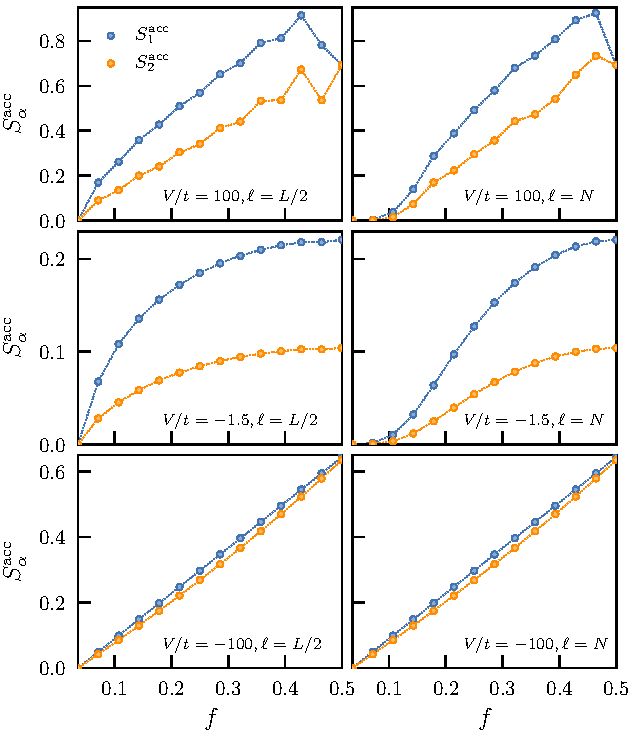
\includegraphics{fillingFractionDependence}
				
	\subsection{}		
		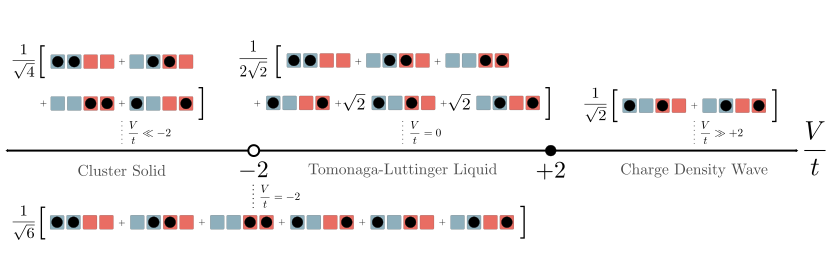
\includegraphics{phaseDiagramTV}
				





	
